% \section{Creating C++ Applications}
\section{Cr\'eer des applications en C++}

% Not everyone wants a full blown GIS desktop application. Sometimes you want
% to just have a widget inside your application that displays a map while the
% main goal of the application lies elsewhere. Perhaps a database frontend with
% a map display? This Section provides two simple code examples by Tim Sutton. 
% They are available in the qgis subversion repository together with more
% interesting tutorials. Check out the whole repository from: 
% \filename{https://svn.osgeo.org/qgis/trunk/code\_examples/}
Pas tout le monde d\'esire une application SIG compl\`ete. Pafois vous voulez juste
un widget inclus dans votre application qui affiche une carte alors que le but 
principal de l'application porte sur autre chose. Peut-\^etre une interface 
cliente d'une base de donn\'ees avec une carte ? Cette section fournit deux 
exemples simples de code \'ecrit par Tim Sutton. Ils sont disponibles dans le d\'ep\^ot
 de code subversion de QGIS r\'eunis avec d'autres tutoriels int\'eressants. 
 R\'ecup\'erez le d\'ep\^ot complet \`a partir de 
 \filename{https://svn.osgeo.org/qgis/trunk/code\_examples/}

% \subsection{Creating a simple mapping widget}\label{subsec:simple_widget}
\subsection{Cr\'eer un simple widget de cartographie}\label{subsec:simple_widget}

% With this first tutorial we take a little walk through creating a simple mapping
% widget. It won't do anything much - just load a shape file and display it in
% a random colour.
\`A travers ce petit tutoriel nous allons faire un petit tour dans la cr\'eation de
widget simple de cartographie.
% But it should give you an idea of the potential for using QGIS as an embedded
% mapping component. Before we carry on, many thanks to Francis Bolduc who wrote
% the beginnings of this demo. He kindly agreed to make his work generally
% available.
Mais il vous donnera une id\'ee du potentiel de l'utilisation de QGIS comme 
composant de cartographie encapsul\'e. Avant de commencer, un grand merci \`a 
Francis Bolduc qui a \'ecrit le d\'ebut de cette d\'emo. Il a gracieusement accept\'e de
rendre son travail disponible.

% We start with typical adding the neccessary includes for our app:
Nous commen\c{c}ons en ajoutant les inclusions n\'ecessaires pour notre application :

\begin{verbatim}
//
// Inclusions pour QGIS
//
#include <qgsapplication.h>
#include <qgsproviderregistry.h>
#include <qgssinglesymbolrenderer.h>
#include <qgsmaplayerregistry.h>
#include <qgsvectorlayer.h>
#include <qgsmapcanvas.h>
//
// Inclusions pour Qt
//
#include <QString>
#include <QApplication>
#include <QWidget>
\end{verbatim}

% We use QgsApplication instead of Qt's QApplication, and get some added
% benifits of various static methods that can be used to locate library paths
% and so on.
Nous utilisons QgsApplication au lieu de QApplication de Qt et nous obtenons des
b\'en\'efices suppl\'ementaires de diff\'erentes m\'ethodes statiques qui peuvent \^etre
utilis\'ee pour localiser les chemins des biblioth\`eques, etc.

% The provider registry is a singleton that keeps track of vector data provider
% plugins. It does all the work for you of loading the plugins and so on. The
% single symbol renderer is the most basic symbology class. It renders points,
% lines or polygons in a single colour which is chosen at random by default
% (though you can set it yourself). Every vector layer must have a symbology
% associated with it.
Le registre des fournisseurs est un singleton qui garde la trace des extensions 
des fournisseurs de donn\'ees vecteurs. Il r\'ealise tout le travail de chargement 
des extensions, etc. \`a votre place. Le moteur de rendu de symbole simple est la 
classe de symbologie la plus simple. Il r\'ealise un rendu de points, lignes ou 
polygones dans une seule couleur qui est choisie al\'eatoirement par d\'efaut (bien 
que vous pouvez le d\'efinir vous m\^eme). Chaque couche vecteur doit avoir une 
s\'emiologie qui lui est associ\'ee.

% The map layer registry keeps track of all the layers you are using. The
% vector layer class inherits from maplayer and extends it to include
% specialist functionality for vector data.
Le registre de couche de la carte garde la trace de toutes les couches que vous 
utilisez. La classe de la couche vecteur h\'erite de maplayer et l'\'etend pour 
inclure des fonctionnalit\'es sp\'ecialis\'ees pour les donn\'ees vecteurs.

% Finally the mapcanvas is really the nub of the matter. Its the drawable
% widget that our map will be drawn onto.
Enfin, le canevas de la carte est vraiment la partie la plus importante, car c'est le widget 
dans lequel notre carte sera dessin\'ee.

% Now we can move on to initialising our application....
Maintenant nous pouvons nous initialiser notre application ...

\begin{verbatim}
int main(int argc, char ** argv)
{
  // D\'ebut de l'application
  QgsApplication app(argc, argv, true);

  QString myPluginsDir        = "/home/timlinux/apps/lib/qgis";
  QString myLayerPath         = "/home/timlinux/gisdata/brazil/BR_Cidades/";
  QString myLayerBaseName     = "Brasil_Cap";
  QString myProviderName      = "ogr";

\end{verbatim}

% So now we have a qgsapplication and we have defined some variables. Since I
% tested this on the Ubuntu 8.10, I just specified the location of the vector
% provider plugins as being inside the my development install directory. It
% would probaby make more sense in general to keep the QGIS libs in one of the
% standard library search paths on your system (e.g. /usr/lib) but this way
% will do for now.
Nous avons donc maintenant une qgsapplication et d\'efinie des variables. Puisque 
j'ai test\'e cela sur Ubuntu 8.10, j'ai d\'efini la localisation de l'extension 
fournisseur de vecteur comme \'etant dans mon r\'epertoire d'installation pour le 
d\'eveloppement. Cela aurait plus de sens, de garder la biblioth\`eque de QGIS dans 
un des chemins de recherche standard de la biblioth\`eque sur votre syst\`eme (par 
exemple /usr/lib/) mais cette mani\`ere conviendra, pour le moment.

% The next two variables defined here just point to the shapefile I am going to
% be using (and you should substitute your own data here).
Les deux variables suivantes d\'efinies ici pointent vers le shapefile que je vais 
utiliser (et vous devez substituer vos propres donn\'ees ici).

% The provider name is important - it tells qgis which data provider to use to
% load the file. Typically you will use 'ogr' or 'postgres'.
Le nom du fournisseur est important - il indique \`a QGIS quel fournisseur de 
donn\'ees \`a utiliser pour charger le fichier. Habituellement, vous utiliserez
 'ogr' ou 'postgres'.

% Now we can go on to actually create our layer object.
Maintenant nous pouvons avancer sur la v\'eritable cr\'eation de notre objet couche.

\begin{verbatim}
  // Instentie le Registre de Fournisseur
  QgsProviderRegistry::instance(myPluginsDir);
\end{verbatim}

% First we get the provider registry initialised. Its a singleton class so we
% use the static instance call and pass it the provider lib search path. As it
% initialises it will scan this path for provider libs.
D'abord, nous initialisons le registre de fournisseur. Comme c'est une classe 
simple, nous utilisons l'appel de l'instance statique et lui passons le chemin 
de recherche des biblioth\`eques du fournisseur. Lors de son initialisation, il 
scannera ce chemin pour les biblioth\`eques du fournisseur.

% Now we go on to create a layer...
Maintenant nous cr\'eons une couche ...

\begin{verbatim}
  QgsVectorLayer * mypLayer =
      new QgsVectorLayer(myLayerPath, myLayerBaseName, myProviderName);
  QgsSingleSymbolRenderer *mypRenderer = new
QgsSingleSymbolRenderer(mypLayer->geometryType());
  QList <QgsMapCanvasLayer> myLayerSet;

  mypLayer->setRenderer(mypRenderer);
  if (mypLayer->isValid())
  {
    qDebug("Layer is valid");
  }
  else
  {
    qDebug("Layer is NOT valid");
  }

  // Ajout de la couche au registre de couche
  QgsMapLayerRegistry::instance()->addMapLayer(mypLayer, TRUE);
  // Ajout de la couche \`a l'ensemble des couches
  myLayerSet.append(QgsMapCanvasLayer(mypLayer, TRUE));

\end{verbatim}

% The code is fairly self explanatory here. We create a layer using the variables 
% we defined earlier. Then we assign the layer a renderer. When we create a
% renderer, we need to specify the geometry type, which do do by asking the
% vector layer for its geometry type. Next we add the layer to a layerset (which
% is used by the QgsMapCanvas to keep track of which layers to render and in
% what order) and to the maplayer registry. Finally we make sure the layer will be
% visible.
Le code est assez explicite ici. Nous cr\'eons une couche en utilisant les variables
que nous avons d\'efinies plus t\^ot. Puis nous assignons \`a la couche un moteur de 
rendu. Lorsque nous cr\'eons un moteur de rendu, nous avons besoins de d\'efinir le 
type de g\'eom\'etrie, ce qui est fait en demandant \`a la couche son type de g\'eom\'etrie.
Puis nous ajoutons la couche \`a un ensemble de couches (qui est utilis\'e par 
QgsMapCanvas pour garder en m\'emoire quelles couches doivent \^etre affich\'ees et 
dans quel ordre) et au registre maplayer. Enfin, nous nous assurons que la couche
 sera visible.

% Now we create a map canvas on to which we can draw the layer.
Maintenant nous cr\'eons un cadre de carte dans lequel nous pouvons dessiner la 
couche.

\begin{verbatim}
  // Creer le cadre de la carte
  QgsMapCanvas * mypMapCanvas = new QgsMapCanvas(0, 0);
  mypMapCanvas->setExtent(mypLayer->extent());
  mypMapCanvas->enableAntiAliasing(true);
  mypMapCanvas->setCanvasColor(QColor(255, 255, 255));
  mypMapCanvas->freeze(false);
  // Definir l'ensemble des couches du cadre de carte
  mypMapCanvas->setLayerSet(myLayerSet);
  mypMapCanvas->setVisible(true);
  mypMapCanvas->refresh();

\end{verbatim}

% Once again there is nothing particularly tricky here. We create the canvas
% and then we set its extents to those of our layer. Next we tweak the canvas a bit
% to draw antialiased vectors. Next we set the background colour, unfreeze the
% canvas, make it visible and then refresh it.
Une fois encore il n'y a rien de particuli\`erement difficile ici. Nous cr\'eons le 
cadre et nous lui d\'efinissons son \'etendue \`a celui de la couche. Puis nous 
modifions l\'eg\`erement le cadre pour dessiner les vecteurs antiali\'es\'es. Enfin, nous 
d\'efinissons la couleur d'arri\`ere-plan, d\'ebloquons le cadre, le rendons visible 
et le rafraichissons.

\begin{verbatim}
  // Debut de la boucle d'evenement de l'application
  return app.exec();
}

\end{verbatim}

% In the last step we simply start the Qt event loop and we are all done. You
% can check out, compile and run this example using cmake like this:
\`A la derni\`ere \'etape, nous d\'emarrons simplement la boucle \'ev\'enementielle de Qt et 
c'est termin\'e. Vous pouvez v\'erifier, compiler et lancer cet exemple en 
utilisant cmake comme ceci :

\begin{verbatim}
svn co
https://svn.osgeo.org/qgis/trunk/code_examples/1_hello_world_qgis_style
cd 1_hello_world_qgis_style
mkdir build
#en option specifiez o\`u QGIS est installe (doit fonctionner sur toutes les plateformes)
#si QGIS est installe dans /usr ou /usr/local vous pouvez laisser tomber l'etape suivante
export LIB_DIR=/home/timlinux/apps
cmake ..
make
./timtut1
\end{verbatim}

% When we compile and run it here is what the running app looks like:
Lorque nous le compilons et le lan\c{c}ons voici ce \`a quoi ressemble l'application lanc\'ee :
\begin{figure}[ht]
   \begin{center}
%    \caption{Simple C++ Application \osxcaption}\label{fig:cpp1_application}\smallskip
   \caption{Application simple en C++ \osxcaption}\label{fig:cpp1_application}\smallskip
   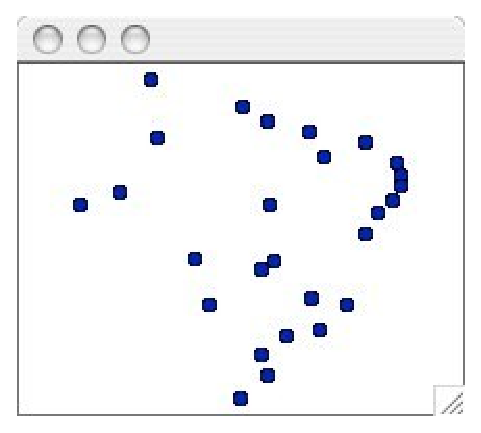
\includegraphics[clip=true]{cpp1_application}
\end{center}
\end{figure}

% \subsection{Working with QgsMapCanvas}
\subsection{Utiliser QgsMapCanvas}

% In Section~\ref{subsec:simple_widget} we showed you the usage of the
% QgsMapCanvas api to create a simple application that loads a shapefile and
% displays the points in it. But what good is a map that you can't interact
% with? 
Dans la section~\ref{subsec:simple_widget} nous vous avons montr\'e l'utilisation 
de l'api QgsMapCanvas pour cr\'eer une application simple qui charge un shapefile 
et affiche les points. Mais \`a quoi sert une carte si vous ne pouvez pas 
interagir avec ?

% In this second tutorial I will extend the last tutorial by making it a
% QMainWindow application with a menu, toolbar and canvas area. We show you how
% to use QgsMapTool - the base class for all tools that need to interact with
% the map canvas.
Dans cette seconde partie, j'\'etendrais la premi\`ere en faisant une application 
QMainWindow avec un menu, une barre d'outils et une zone de carte. Nous vous 
avons montr\'e comment utiliser QgsMapTool - la classe de base pour tous les 
outils qui n\'ecessite d'interagir avec le cadre de carte.
% The purpose is to provide a demonstrator project, so I wont promise to write the most
% elegant or robust C++ code. The project will provide 4 toolbar icons for
Le but est de fournir un projet de d\'emonstration, je ne promets donc pas d'\'ecrire
 le code C++ le plus robuste et le plus \'el\'egant. Le projet fournira 4 ic\^ones de 
 barres d'outils.

\begin{itemize}
%  \item loading a map layer (layer name is hard coded in the application
  \item charger une carte (le nom de la couche est cod\'e en dur dans l'application)
%  \item zooming in
  \item d\'ezoomer
%  \item zooming out
  \item zoomer
%  \item panning
  \item d\'eplacer
\end{itemize}

% In the working directory for the tutorial code you will find a number of files
% including c++ sources, icons and a simple data file under data. There is also
% the .ui file for the main window.
Dans le r\'epertoire de travail du code de ce cours, vous trouverez quelques 
fichiers incluant les sources c++, des ic\^ones et un fichier de donn\'ees simple 
dans le r\'epertoire data. Il y a aussi des fichiers .ui pour la fen\^etre principale.

% \textbf{Note:} You will need to edit the .pro file in the above svn directory to
% match your system.
\textbf{Note :} vous aurez besoin d'\'editer lefichier .pro dans le r\'epertoire svn 
ci-dessus pour qu'il corresponde \`a votre syst\`eme.

% Since much of the code is the same as the previous tutorial, I will focus on
% the MapTool specifics - the rest of the implementation details can be
% investigated by checking out the project form SVN. A QgsMapTool is a class that
% interacts with the MapCanvas using the mouse pointer. QGIS has a number of
% QgsMapTools implemented, and you can subclass QgsMapTool to create your own. In
% mainwindow.cpp you will see I include the headers for the QgsMapTools near the
% start of the file:
Puisqu'une grande partie du code est le m\^eme que la partie pr\'ec\'edente, nous nous
focaliserons sur les sp\'ecificit\'es de MapTool - le reste des d\'etails de 
l'impl\'ementation peut \^etre regard\'e en r\'ecup\'erant le projet \`a partir du SVN. Un 
QgsMapTool est une classe qui interagit avec le MapCanvas en utilisant le pointeur
 de la souris. QGIs a un certain nombre de QgsMapTools impl\'ement\'e, et vous 
 pouvez sous-classer QgsMapTool pour cr\'eer les v\^otres. Dans le fichier 
 mainwindow.cpp vous verrez que j'ai inclus les en-t\^etes pour QgsMapTools pr\`es 
 du d\'ebut du fichier :
\begin{verbatim}
     //
     // QGIS Map tools
     //
     #include "qgsmaptoolpan.h"
     #include "qgsmaptoolzoom.h"
     //
     // Il y a d'autres en tete pour les outils de la carte disponibles
     // (non utilise dans cet exemple)
     //
     //#include "qgsmaptoolcapture.h"
     //#include "qgsmaptoolidentify.h"
     //#include "qgsmaptoolselect.h"
     //#include "qgsmaptoolvertexedit.h"
     //#include "qgsmeasure.h"
\end{verbatim}

% As you can see, I am only using two types of MapTool subclasses for this
% tutorial, but there are more available in the QGIS library. Hooking up our
% MapTools to the canvas is very easy using the normal Qt4 signal/slot mechanism:
Comme vous pouvez le voir, je n'utilise que deux types de sous-classe MapTool 
pour cette partie, mais il y en a plus de disponibles dans la biblioth\`eque QGIS.
Agrafer notre MapTools au cadre est tr\`es facile en utilisant le m\'ecanisme normal 
slot/signal de Qt4.

\begin{verbatim}
     //creer le comportement action
     connect(mActionPan, SIGNAL(triggered()), this, SLOT(panMode()));
     connect(mActionZoomIn, SIGNAL(triggered()), this, SLOT(zoomInMode()));
     connect(mActionZoomOut, SIGNAL(triggered()), this, SLOT(zoomOutMode()));
     connect(mActionAddLayer, SIGNAL(triggered()), this, SLOT(addLayer()));
\end{verbatim}

% Next we make a small toolbar to hold our toolbuttons. Note that the mpAction*
% actions were created in designer.
Puis nous r\'ealisons une barre d'outils pour contenir nos boutons. Notez que les 
actions mpAction* ont \'et\'e cr\'e\'ees dans QtDesigner.

\begin{verbatim}
     //creer une petite barre d'outils
     mpMapToolBar = addToolBar(tr("File"));
     mpMapToolBar->addAction(mpActionAddLayer);
     mpMapToolBar->addAction(mpActionZoomIn);
     mpMapToolBar->addAction(mpActionZoomOut);
     mpMapToolBar->addAction(mpActionPan);
\end{verbatim}

% Thats really pretty straightforward Qt stuff too. Now we create our three map
% tools:
Ceci \'egalement est une possibilit\'e de Qt assez simple.Maintenant nous cr\'eons 
nos trois outils pour la carte :

\begin{verbatim}
     //creer les outils de le carte
     mpPanTool = new QgsMapToolPan(mpMapCanvas);
     mpPanTool->setAction(mpActionPan);
     mpZoomInTool = new QgsMapToolZoom(mpMapCanvas, FALSE); // false = in
     mpZoomInTool->setAction(mpActionZoomIn);
     mpZoomOutTool = new QgsMapToolZoom(mpMapCanvas, TRUE ); //true = out
     mpZoomOutTool->setAction(mpActionZoomOut);
\end{verbatim}

% Again nothing here is very complicated - we are creating tool instances, each
% of which is associated with the same mapcanvas, and a different QAction. When
% the user selects one of the toolbar icons, the active MapTool for the canvas is
% set. For example when the pan icon is clicked, we do this:
Rien de bien compliqu\'e ici aussi - nous cr\'eons des instances d'outils, chacune 
d'elles est associ\'ee avec le m\^eme mapcanvas, et une QAction diff\'erente. Quand 
l'utilisateur s\'electionne une des ic\^ones de la barre d'outils, le MapTool actif 
pour le canevas est d\'efini. Par exemple quand l'ic\^one d\'eplacement est cliqu\'ee, 
nous r\'ealisons cela :

\begin{verbatim}
    void MainWindow::panMode()
    {
       mpMapCanvas->setMapTool(mpPanTool); 
    }
\end{verbatim}

\begin{figure}[ht]
   \begin{center}
%    \caption{QMainWindow application with a menu, toolbar and canvas area
   \caption{Application QMainWindow avec un menu, une barre d'outils et une zone de carte
\osxcaption}\label{fig:cpp2_application}\smallskip
   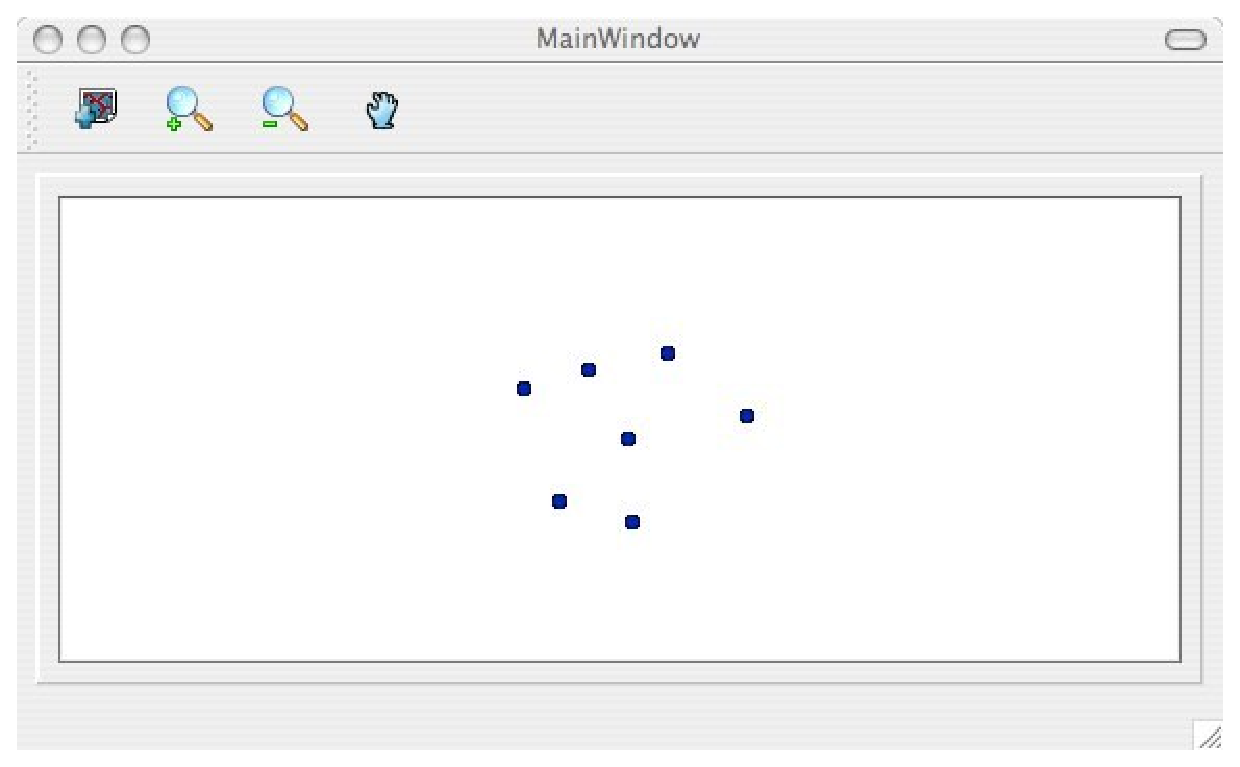
\includegraphics[clip=true, width=\textwidth]{cpp2_application}
\end{center}
\end{figure}

% \minisec{Conclusion}
\minisec{Conclusion}

% As you can see extending our previous example into something more functional
% using MapTools is really easy and only requires a few lines of code for each
% MapTool you want to provide.
Comme vous pouvez le voir, \'etendre notre exemple pr\'ec\'edent en quelque chose de 
plus fonctionnel en utilisant MapTools est vraiment facile et n\'ecessite 
seulement quelques lignes de codes pour chaque MapTool que vous voulez fournir.

% You can check out and build this tutorial using SVN and CMake using the following steps:
Vous pouvez r\'ecup\'erer et compiler ce tutoriel en utilisant SVN et CMake avec 
les \'etapes suivantes :

\begin{verbatim}
svn co https://svn.osgeo.org/qgis/trunk/code_examples/2_basic_main_window
cd 2_basic_main_window
mkdir build
#en option sp\'ecifiez o\`u QGIS est installe (doit fonctionner sur toutes les plateformes)
#si QGIS est installe dans /usr ou /usr/local vous pouvez laisser tomber l'\'etape suivante
export LIB_DIR=/home/timlinux/apps
cmake ..
make
./timtut2
\end{verbatim}
